Podstawowym problemem w użytkowaniu zdalnych aplikacji niezależnie od protokołu jest ilość przesłanych danych oraz opóźnienie. Przeprowadzono proste testy porównujące pod tym względem stworzone rozwiązanie z systemem \emph{VNC}. Porównanie to nie jest bardzo dokładne i przedstawione dane są jedynie poglądowe. Pełna analiza wymaga dokładnego poznania protokołu \emph{RFB}, który wykorzystuje \emph{VNC} i modyfikacji obecnych klientów w celu zebrania danych diagnostycznych.

Specyfikacja sprzętowa.
\begin{itemize}
\item Klient oraz maszyna lokalna -- procesor Intel Core i5-2400, 8GB pamięci RAM, dysk SSD.
\item Serwer zdalny -- VPS (ang. Virtual Private Server), procesor Intel Core i5-3570K z dostępem do 2 rdzeni, 2GB pamięci RAM, współdzielony dysk SSD.
\end{itemize}

Specyfikacja oprogramowania.
\begin{itemize}
\item Klient oraz maszyna lokalna --- openSUSE Linux 12.1, Qt 4.7.4, KDE 4.7.2, klient VNC TightVNC Viewer 1.3.10, Mozilla Firefox 17.0.1.
\item Serwer zdalny --- Debian Unstable, Qt 4.8.2, KDE 4.8.4, serwer VNC TightVNC Server 1.3.9.
\end{itemize}

Na obu komputerach oprogramowanie zostało zainstalowane w standardowy sposób oraz nie dokonywano żadnych zmian w ustawieniach. Używany jest domyślny styl \emph{Oxygen}.

Do porównania wybrano dwa programy -- kalkulator \emph{KCalc} dostępny w podstawowym pakiecie KDE oraz grę pasjans \emph{KPat} (aka \emph{KPatience}) z pakietu KDE Games. \emph{KCalc} jest aplikacją wykorzystującą podstawowe widgety, gdzie praktycznie nie używane są bitmapy. Gra \emph{KPat} prawie w całości bazuje na elemencie, który w \emph{Qt} renderowany jest za pomocą bitmap. Wybór tych programów pozwoli na porównanie działania dla dwóch różnych przypadków --- dużej ilości natywnych widgetów albo dużej ilości grafik.

\section {Testy funkcjonalne}
Z powodu poziomu skomplikowania aplikacji testy funkcjonalne przeprowadzono ręcznie. Polegały na uruchomieniu wielu programów użytkowych z pakietu \emph{KDE} takich jak:
\begin{itemize}
\item \emph{KCalc},
\item \emph{Dolphin},
\item \emph{QtCreator},
\item \emph{KPat},
\item \emph{Kwrite},
\item \emph{Konsole}.
\end{itemize}

Aplikacje były sprawdzane pod względem poprawności wyświetlania elementów, funkcjonalności menadżera okien i możliwości interakcji użytkownika. Przykładowe aplikacje uruchomione przy pomocy projektu przedstawione są na rysunkach \ref{dolphin}, \ref{qtcreator} oraz \ref{konsole}.

\begin{figure}[H]
  \centering
  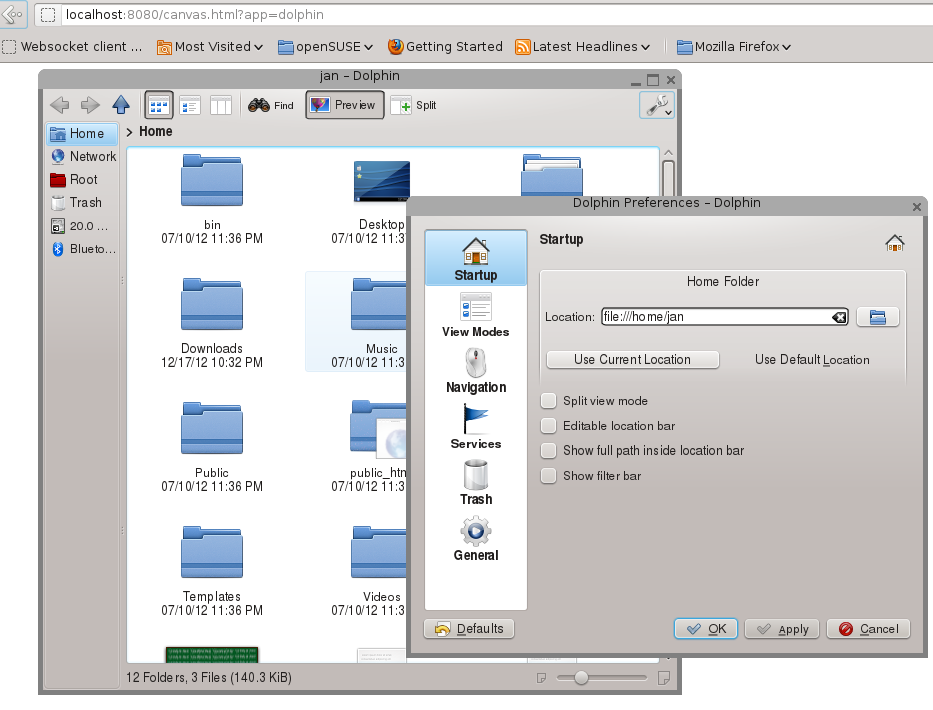
\includegraphics[width=\textwidth,height=!]{img/dolphin.png}
  \caption{Aplikacja \emph{Dolphin}}
  \label{dolphin}
\end{figure}


\begin{figure}[H]
  \centering
  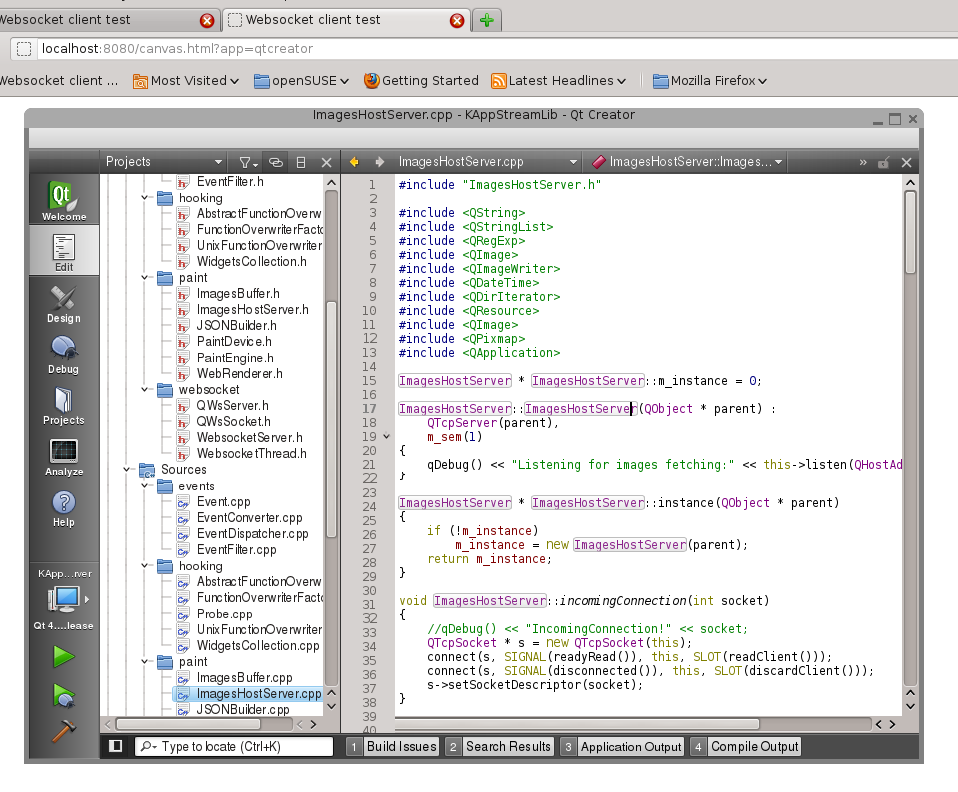
\includegraphics[width=\textwidth,height=!]{img/qtcreator.png}
  \caption{Aplikacja \emph{QtCreator}}
  \label{qtcreator}
\end{figure}

\begin{figure}[H]
  \centering
  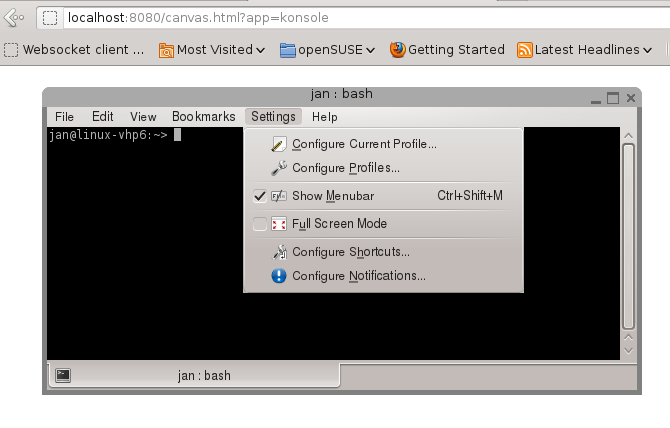
\includegraphics[width=\textwidth,height=!]{img/konsole.png}
  \caption{Aplikacja \emph{Konsole}}
  \label{konsole}
\end{figure}

\section{Testy wydajnościowe}

\subsection{Badanie ilości przesłanych danych}

Stworzono dwa przypadki testowe wykonane w 5 próbach. Pierwszy polega na włączneniu aplikacji i pomiarze przesłanych danych aż do pełnego wyświetlenia się na ekranie. Wyniki znajdują się w tablicach \ref{tab:test1} oraz \ref{tab:test2}. Drugim scenariuszem jest sprawdzenie działania aplikacji w dłuższym okresie czasu. Dokonano nagrania prostego makra z użyciem myszy za pomocą aplikacji \emph{xmacro2}. Testu dokonywano przez około minutę testując cykliczne kliknięcia na wybranych elementach w stałych odstępach czasu. Wyniki dostępne w tablicach \ref{tab:test3} oraz \ref{tab:test4}.

Wyniki wskazują wyższość systemu \emph{VNC} pod kątem ilości przesłanych danych. Różnice te wynikają przede wszystkim z narzutu protokołu. \emph{RFB} jest protokołem binarnym, gdzie przesyłane są głównie obrazy. W protokole użytym w projekcie duży narzut stanowi użyty format \emph{JSON}. Obejściem tego problemu może być próba zastosowanie kompresji \emph{GZIP}. Przesyłane dane ze względu na ogarniczoną ilość użytych znaków, które często się powtarzają bardzo dobrze się kompersują -- uzyskiwany jest kilkukrotny zysk objętościowym. Za pomocą \emph{WebWorkerów HTML5} możliwa jest dekompresja w wielu wątkach w celu przyspieszenia aplikacji.

\begin{table}
\centering  
\begin{tabular}{l*{6}{|c}r}
\multicolumn{7}{c}{KCalc} \\
\hline
Aplikacja              & 1 & 2 & 3 & 4 & 5  & Średnia  \\
\hline
KAppstream & 560 & 1002 & 494 & 506 & 641 &  640  \\
\hline
VNC            & 592 & 621 & 651 & 575 &  584 &  604  \\
\end{tabular}
\caption{Test aplikacji \emph{KCalc} -- ilość przesłanych danych od startu}
\label{tab:test1}
\end{table}

\begin{table}
\centering  
\begin{tabular}{l*{6}{|c}r}
\multicolumn{7}{c}{KPat} \\
\hline
Aplikacja              & 1 & 2 & 3 & 4 & 5  & Średnia  \\
\hline
KAppstream & 672 & 642 & 694 & 705 & 650 &  672  \\
\hline
VNC            & 619 & 981 & 651 & 575 &  610 &  687  \\
\end{tabular}
\caption{Test aplikacji \emph{KPat} -- ilość przesłanych danych od startu}
\label{tab:test2}
\end{table}


\begin{table}
\centering  
\begin{tabular}{l*{6}{|c}r}
\multicolumn{7}{c}{KCalc} \\
\hline
Aplikacja              & 1 & 2 & 3 & 4 & 5  & Średnia  \\
\hline
KAppstream & 1802 & 2021 & 1902 & 2104 & 1802 &  1926  \\
\hline
VNC            & 1021 & 989 & 1101 & 1021 &  1258 &  1078  \\
\end{tabular}
\caption{Test działania aplikacji \emph{KCalc}  -- symulacja działania użytkownika}
\label{tab:test3}
\end{table}

\begin{table}
\centering
\begin{tabular}{l*{6}{|c}r}
\multicolumn{7}{c}{KPat} \\
\hline
Aplikacja              & 1 & 2 & 3 & 4 & 5  & Średnia  \\
\hline
KAppstream & 10847 & 9054 & 10814 & 9581 & 10485 & 10156   \\
\hline
VNC            & 6945 & 7541 & 6801 & 6541 &  7211 & 7007   \\
\end{tabular}
\caption{Test działania aplikacji \emph{KPat} -- symulacja działania użytkownika}
\label{tab:test4}
\end{table}

\subsection{Badanie działania przy słabym połączeniu i dużych opóźnieniach}

Do symulacji pracy przy użyciu słabego łącza wykorzystano pakiet netem \cite{netem}. Z powodu braku możliwości łatwego opisania konkretnymi wartościami testów zapisano jedynie odczucia z punktu widzenia użytkownika. Przeprowadzono dwa testy.

Pierwszy test miał na celu sprawdzenie funkcjonalność przy niewielkim opóźnieniu około 100 milisekund przy stracie pakietów około 0.3\%. Zastosowano następujące polecenia:\\
\texttt{tc qdisc change dev eth0 root netem delay 100ms 20ms distribution normal} \\
\texttt{tc qdisc change dev eth0 root netem loss 0.3\% 50\%} \\ 
W takich warunkach testowana aplikacja zachowywała się prawidłowo. Opóźnienia i responsywność nie odbiegały wiele od systemu \emph{VNC}.

Drugi test badał zachowanie funkcjonalności przy zastosowaniu bardzo słabego łącza. Zasymulowano opóźnienie około 600 milisekund i stratę pakietów na poziomie 1\%. Zastosowano następujące polecenia: \\
\texttt{tc qdisc change dev eth0 root netem delay 600ms 50ms distribution normal} \\
\texttt{tc qdisc change dev eth0 root netem loss 1\% 50\%} \\ 
W takiej sytuacji testowana aplikacja zachowywała się prawidłowo i była w pełni stabilna. Reagowała na aktywność użytkownika prawidłowo i mimo spowolnienia w wyświetlaniu nie zaobserwowano znaczących błędów i awarii serwera.
Mimo tego z powodu zbyt dużego obciążenia z punktu widzenia użytkownika aplikacje uruchomina za zarówno w testowanym systemie jak i w \emph{VNC} były bardzo niewygodne w użytkowaniu. Nie zauważono dużych różnic w działaniu obu rozwiązań w tej próbie.

\section{Podsumowanie testów}
W środowisku lokalnym oba rozwiązania praktycznie nie różnią się od siebie w kwestii wydajności. Przewaga systemu \emph{VNC} w sieci Internet wynika głównie z powodu mniejszej ilości przesyłanych danych. Przy zastosowaniu dodatkowych rozwiązań kompresujących dane możliwe będzie uzyskanie wyniku zbliżonego, lub nawet niższego w szczególnych przypadkach.
Nowoczesne przeglądarki bardzo dobrze radzą sobie z rysowaniem. Dla testowanej przeglądarki \emph{Mozilla Firefox} czas rysowania na elemencie \emph{canvas} jest wartością całkowicie pomijalną. Rysowanie jednego widgeta trwa około 1-3 milisekund, w zależności od poziomu skomplikowania. Pomiarów tych dokonano przy pomocy metody \emph{Date.getTime()}.